\documentclass[a4paper]{article}

\usepackage[english]{babel}
\usepackage[utf8]{inputenc}
\usepackage{amsmath}
\usepackage{graphicx}
\usepackage[colorinlistoftodos]{todonotes}

\title{Solar cell}

\author{The authors}

\date{\today}

\begin{document}
\maketitle

\section{Introduction}

A solar cell is an eletrical device that generates electricity by the photovoltaic effect. Upon exposure to illumination, the device creates voltage, which in turn gives rise to an electric current. Solar cells are becoming increasingly common as an alternative source of electricity. \\

A solar cell can be described as a $p-n$ junction, which is an interface between $p$-type material (acceptors) and $n$-type material (donors) inside a semiconductor. Electrons will diffuse from the $n$-side to the $p$-side, while holes will diffuse from the $p$-side to the $n$-side. At the same time, an electric field comes into existance between the diffused electrons at the $p$-side and the diffused holes at the $n$-side. Whereas the diffusion force pulls electrons to the $n$-side and holes to the $p$-side, the force from the built-in electric field will pull both electrons and holes in the opposite direction, counteracting the diffusion. Sooner or later the forces will be equal, and an equilibrium is established. \\

%\begin{figure}[h]
%\centering
%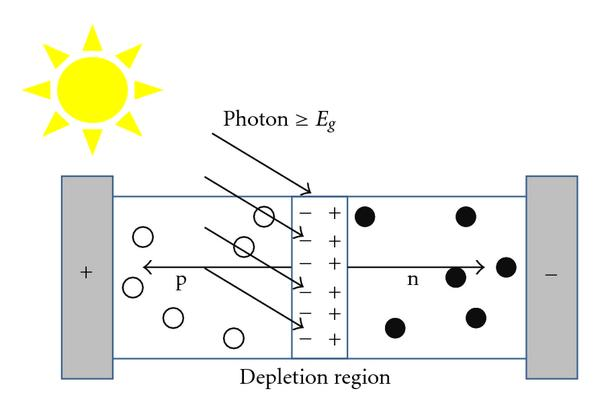
\includegraphics[width=\textwidth]{solarcell.jpg}
%\caption{Basic p-n junction solar cell and charge transport phenomena. (Change description.)}
%\label{fig:solarcell}
%\end{figure}

Free electron-hole pairs can be generated in a semiconductor when it is exposed to light with sufficient energy to excite electrons to the conduction band. If this happens close enough to the interface between the two sides, the electron and hole will feel the built-in electric field, and will consequently be swept in different directions. When the sides are shortcircuited, electrons will flow from the $n$-side to the $p$-side to recombine with the holes. This is how solar cells generate an electric current. Note that the direction is the opposite of a diode, because we have minority carriers instead of majority carriers.

\section{Experimental procedure}

The solar cell we used in this laboration is a polycrystalline silicon thin film. The area of the solar cell was $2.3 \times 6.0$ cm$^2$. A $60$ W standard desk lamp provided the illumination.

\section{Measurement results}

Diagrams... Fit to the diode equation $I = I_{sat}\left(1-\exp\left(-\frac{eV}{nk_BT}\right)\right)$, where $n$ is the ideality factor.

\section{Discussion of the results}

Not exactly as expected. The correlation should obey $4\pi R^2\Phi = P$, where $P$ is the effect. (We measured the maximal effect $P_{max}$).

\section{Conclusions}

It works.

\end{document}
